\documentclass{article}
\usepackage{tikz}

\begin{document}

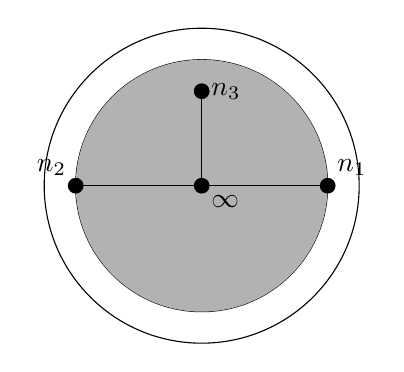
\begin{tikzpicture}[scale=2]
    % Draw the large circle
    \draw (0,0) circle (1);
    
    % Draw the smaller circles
    \draw (0,0) circle (0.8);
    \draw (0,0) circle (0.6);
    
    % Draw the shaded region
    \fill[black!30] (0,0) circle (0.8);
    \fill[black!30] (0,0) circle (0.6);
    
    % Label the points
    \fill (0,0) circle (0.05) node[below right] {$\infty$};
    \fill (0.8,0) circle (0.05) node[above right] {$n_1$};
    \fill (-0.8,0) circle (0.05) node[above left] {$n_2$};
    \fill (0,0.6) circle (0.05) node[right] {$n_3$};
    
    % Draw the lines connecting the points to the center
    \draw (0,0) -- (0.8,0);
    \draw (0,0) -- (-0.8,0);
    \draw (0,0) -- (0,0.6);
\end{tikzpicture}

\end{document}